\chapter{Radio electronic characteristics}

By the time the \gls{rf} signal has reached the acoustic transducer, it has
been synthesized from a reference signal, amplified, and matched to the
impedance of the \gls{aod} transducer. We are going to inspect the \gls{rf}
signal characteristics at each transmission and find that each stage
unintentionally carries out frequency dependent amplitude modulation which,
as we will see in the next chapter, is responsible for the complex intensity
distribution observed with the photodiode.

\section{Digital signal synthesizer}

We already covered the fundamental functionality of the \gls{dds} in XX and
its integration in our experimental setup in YY, yet we are missing physical
measurements.

Physical analysis of the \gls{dds} output \gls{rf} signal is in fact no
simple endeavour as usual operation time scales are of many magnitudes
greater than the signal periodicity. The strategy we used to resolve this
circumstance is depcited in \Cref{fig:dds_sweep_window}. The strategy
consists of capturing multiple, small time windows of the signal which
delayed would cover the complete signal trace.

\begin{figure}[h]
  \centering
  \includegraphics[width=\textwidth]{\mediadir{diagram/sweep-window.pdf}}
  \captionsetup{width=.8\textwidth}
  \caption{Idealized \gls{dds} signal output with constant frequency and
    linear ramp over the sweep duration. The measured window only captures
    a subset of the complete sweep but can be delayed to cover the complete
    sweep duration.}
  \label{fig:dds_sweep_window}
\end{figure}

The experimental setup is schematically drawn in
\Cref{fig:dds_sweep_window_setup}. In between the oscilloscope and the
trigger source we inserted a pulse generator. The pulse generator width
corresponds to the delay time of the oscilloscope as the oscilloscope is
configured to capture on the falling edge signal of the pulse generator.

\begin{figure}[h]
  \centering
  \includegraphics[width=\textwidth]{\mediadir{setup/sweep-window.pdf}}
  \captionsetup{width=.8\textwidth}
  \caption{By inserting a pulse generator in between the trigger source and
  the oscilloscope we can delay the capture window of the oscilloscope by
the pulse width.}
  \label{fig:dds_sweep_window_setup}
\end{figure}

In \Cref{tab:dds_signal_parameters} we can find an overview of the
experimental parameters.

\begin{table}[h]
  \centering
  \begin{tabular}{|c|c|c|c|c|}
    \hline
    Start frequency $f_0$ &
    Final frequency $f_1$ &
    Sweep duration $T_s$ &
    Window duration $T_w$ \\
    \hline
    \SI{80}{\mega\hertz} &
    \SI{4.88}{\mega\hertz} &
    \SI{200.00}{\micro\second} &
    \SI{26.84}{\milli\second} \\
    \hline
  \end{tabular}
  \captionsetup{width=.8\textwidth}
  \caption{Experimental parameters used to inspect the output \gls{rf} signal
  of the \gls{dds}.}
  \label{tab:dds_signal_parameters}
\end{table}

The specified frequency range is motivated to cover
the greatest possible spatial dimensions permitted by the dimensions of the
optics. Sweep and window duration where selected as a compromise between the
oscilloscope being able to resolve the signal fine enough to perform
\gls{fft} and the sweep duration being comparable to later experiments. Time
delay between windows was choosen to be $T_s/300$, thus we will capture 300
overlapping time windows.

\subsection{Discrete frequency spectrum}

For an ideal linear frequency sweep we would expect a continous increase of
the frequency with respect to time, yet we know that \gls{dds} makes use of
digital signal processing methods which suggests a discrete frequency
spectrum. To help us expose the characteristics of the digital frequency
sweep we will utilize a spectrogram. A spectrogram visualizes how the
frequency spectrum varies in time. One way to obtain a spectrogram is to
partition the data into overlapping time chunks while performing \gls{fft}
which allows us to combine time and frequency domain specific
characteristics. In our case we choose the relative spectral power to be
encoded through color.

\begin{figure}[h]
  \centering
  \includegraphics[width=\textwidth]{\figuredir{signal/synthesis/spectrogram.pdf}}
  \captionsetup{width=.8\textwidth}
  \caption{Spectrogram of delayed time windows of the \gls{dds} output signal
    configured to perform a linear frequency sweep. For an ideal linear sweep
    we would expect a linear timeline of the frequency, instead we observe a
    discrete set of frequencies.}
  \label{fig:signal_synthesis_spectrogram}
\end{figure}

\Cref{fig:signal_synthesis_spectrogram} depicts four spectrograms, each taken
at a different time window of the frequency sweep passthrough. The first
spectrogram captures the start of the frequency sweep. We can see how for the
first \SI{200}{\micro\second} the \gls{dds} outputs only the start frequency
of \SI{80}{\mega\hertz} which then is increased by increments to reach the
final frequency of \SI{120}{\mega\hertz} as can be seen in the lower right
spectrogram at the end of the frequency sweep.

\subsection{Amplitude frequency response}

Although the previous section satisfied our curiousity, it did only confirm
made presumptions. We will now move on with the examination of the amplitude
frequency response which by all means shows unexpected behaviour.

In the Fourier space we can locate the dominant frequency at the maximum of
the power spectrum. That in mind we can reduce the previous obtained time
window measurements to pairs of dominant frequency and maximum amplitude.
Under the assumption that the maximum amplitude lies closely in range of the
mean amplitude we find the amplitude frequency response spectrum.

\begin{figure}[h]
  \centering
  \includegraphics[width=.9\textwidth]{\figuredir{signal/synthesis/inverse-sinc.pdf}}
  \captionsetup{width=.9\textwidth}
  \caption{Maximum amplitude of the \gls{dds} signal output at different
    frequencies during linear sweep operation. In the bottom trace the
    \gls{dds} was configured with enabled inverse-sinc filter.}
  \label{fig:signal_synthesis_inverse_sinc}
\end{figure}

\Cref{fig:signal_synthesis_inverse_sinc} visualized the previously described
routine for the \gls{dds} assigned to the vertical \gls{aod}. The data
trace for the horizontal \gls{dds} is of equal shape, thus there are no
differences between the output signals of distinct \gls{dds} and we can limit
ourselves to the analysis of one such output. In
\Cref{fig:signal_synthesis_inverse_sinc} we can see a strong frequency
response of the amplitude. In particular we observe that at around
\SI{80}{\mega\hertz} and \SI{103}{\mega\hertz} the amplitude shows
significant local minima. The datasheet of the \gls{ad9910} reports a
characteristic sinc dependency of the output power \cite{AD9910} and thus
promotes a built-in inverse-sinc filter to compensate in respect thereof.
Having said that the reported output power in dependency of the frequency
in \cite{AD9910} should only be of linear order for the investigated
frequency range and in fact as we can see in the lower trace in
\Cref{fig:signal_synthesis_inverse_sinc} the enabled inverse-sinc filter
does not account for our observed amplitude response.

\begin{figure}[h]
  \centering
  \includegraphics[width=.9\textwidth]{\figuredir{signal/synthesis/csample-dramp.pdf}}
  \captionsetup{width=.9\textwidth}
  \caption{Maximum amplitude of the \gls{dds} signal output at different
    frequencies once obtained by linear sweep operation and once through
    manual frequency sampling.}
  \label{fig:signal_synthesis_scample_dramp}
\end{figure}

One hypothesis suggested that the observed amplitude response is caused by
fact that the frequencies are sampled internally from the digital ramp logic.
Therefore we collected second data where we configured the vertical \gls{dds}
to output constant frequencies. The amplitude response for this setup is
disclosed in \Cref{fig:signal_synthesis_scample_dramp}. We can see that
indeed the digital ramp introduces a small frequency shift, nonetheless it
still shows the same global behaviour of the output power. Therefore we are
left unanswered with the origin of the observed output power spectrum.

\section{Amplifier}

\subsection{Transmission spectrum}

\subsection{Amplitude frequency response}

\section{Acoustic transducer}

\subsection{Reflection spectrum}
